As we have already said, we had to design a framework in such a way that our algorithms can share and exploit specific functionalities. In this context, it becomes useful to give a general view of the whole system by identifying and defining its abstraction layers, as shown in Figure~\ref{levels}. Let's briefly comment each of this levels and then focus on their specific features.
\begin{figure}[h]
  \begin{center}
    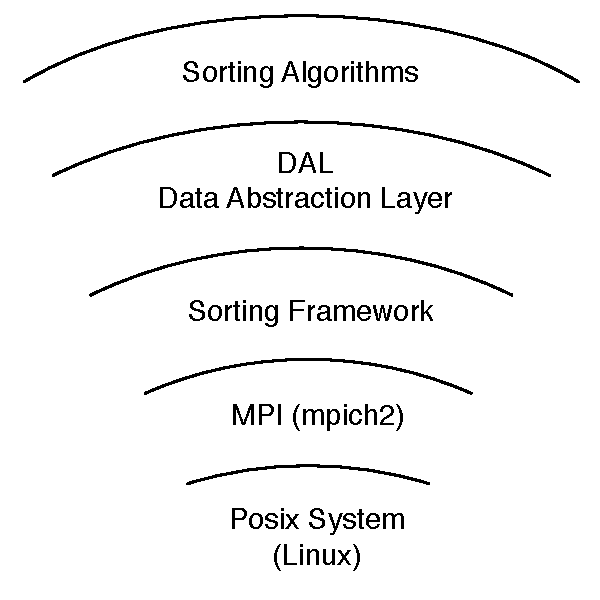
\includegraphics[scale=0.60]{levels}
  \end{center} 
  \caption{Abstract model}
  \label{levels}
\end{figure}
\begin{enumerate}
\item \textbf{Sorting Algorithms.} The logic of a parallel sorting algorithm is defined at this level. The programmer works on primitives and data types provided by the DAL. It should be obvious, but we want to stress the fact that no visibility of MPI is provided at this level, that is the processes of a parallel algorithm communicate each other thanks to the communication primitives provided by the DAL.  
\item \textbf{Sorting Framework.} At this level we implemented a set of functionalities that are commons and essentials to every sorting algorithm: generation of datas, loading of data sets and storing of results, timing are the most important. 
\item \textbf{Data Abstraction Layer.} The DAL, as it will be better explained in~\ref{DAL}, allows us to decouple the designing of parallel algorithms from the necessity of handling data sets that can not fit the memory. 
\item \textbf{MPI.} It is the communication library between processes that we used to implement the Sorting Framework. In particular we chose a specific implementation, \textit{mpich2}, since it gives us the possibility of managing the deployment of the processes. Indeed, unlike the other implementations of MPI, \textit{mpich2} let us to specificy on which specific node a certain process, with its own specific rank, must be allocated. We will exploit this feature to build, for the same algorithm, different mappings of processes to nodes, in such a way to try to diminish the impact of communications on the performance. 
\item \textbf{Posix System (Linux).} Almost all the upper levels exploit Posix mechanisms, e.g. for gathering times, argument parsing, dynamic loading. This is quite important because Linux becomes the only platform on which is possible to run the application (cygwin remains a secondary option). 
\end{enumerate}
In some sense, we can say that starting from a tool for parallel programming like MPI, we designed a new tool, namely the run-time support of the Sorting Algorithm level, that addresses our needs for implementing parallel sorting algorithm for large data sets. 

In the following we are going to describe each of these levels starting from the top-most one, namely Sorting Algorithms. The emphasis will be obvioulsy put on the firsts layers (Sorting Algorithms, DAL, Sorting Framework) which mainly represent the work we made in this project.

